%% $RCSfile: proj_proposal.tex,v $
%% $Revision: 1.2 $
%% $Date: 2010/04/23 02:40:16 $
%% $Author: kevin $

\documentclass[11pt, a4paper, twoside, openright]{report}

\usepackage{float} % lets you have non-floating floats

\usepackage{url} % for typesetting urls
\usepackage{graphicx}
%  We don't want figures to float so we define
%
\newfloat{fig}{thp}{lof}[chapter]
\floatname{fig}{Figure}

%% These are standard LaTeX definitions for the document
%%
\title{An Investigation into Alternative Solutions to ESPAC for Assessing Earthquake Liquefaction Potential}
\author{George Charles Davie}

%% This file can be used for creating a wide range of reports
%%  across various Schools
%%
%% Set up some things, mostly for the front page, for your specific document
%
% Current options are:
% [ecs|msor]              Which school you are in.
%
% [bschonscomp|mcompsci]  Which degree you are doing
%                          You can also specify any other degree by name
%                          (see below)
% [font|image]            Use a font or an image for the VUW logo
%                          The font option will only work on ECS systems
%
\usepackage[font,ecs]{vuwproject} 

% You should specifiy your supervisor here with
     \supervisor{William Neil L Browne}
% use \supervisors if there are more than one supervisor

% Unless you've used the bschonscomp or mcompsci
%  options above use
\otherdegree{Bachelor of Engineering}
% here to specify degree

% Comment this out if you want the date printed.
\date{}

\begin{document}

% Make the page numbering roman, until after the contents, etc.
\frontmatter

%%%%%%%%%%%%%%%%%%%%%%%%%%%%%%%%%%%%%%%%%%%%%%%%%%%%%%%

\begin{abstract}
   Standard regression techniques for soil analysis are time consuming and subject to human bias. The Institute of Geological and Nuclear Sciences (GNS) and
Victoria University have developed a proof of concept prototype as a solution to this problem, Evolutionary Spatial Auto-Correlation (ESPAC). ESPAC is an implementation of the parallel linear genetic programming (PLGP) algorithm. Due to the nature of this project no alternative solutions were investigated. This project aims to address this issue by investigating the properties of five separate artificial intelligence techniques. The aim to lend strength to the argument that PLGP is the correct solution to the problem, or find that an alternative method would be more viable, all within the time restrictions of a $4^{th}$ year honors project.
\end{abstract}

%%%%%%%%%%%%%%%%%%%%%%%%%%%%%%%%%%%%%%%%%%%%%%%%%%%%%%%

\maketitle

%\tableofcontents

% we want a list of the figures we defined
%\listof{fig}{Figures}

%%%%%%%%%%%%%%%%%%%%%%%%%%%%%%%%%%%%%%%%%%%%%%%%%%%%%%%

\mainmatter

%%%%%%%%%%%%%%%%%%%%%%%%%%%%%%%%%%%%%%%%%%%%%%%%%%%%%%%

\section*{1. Introduction}

Determining the chance of liquefaction within a specific geographic area is an important
task especially in light of the recent Christchurch earthquakes. The current
processes are labor intensive and subject to human error and bias. Developing a processes that would provide accurate reliable results with a reduction in human processing time would be beneficial tool to the geotechnic industry. The benefits include: 
\begin{itemize}
\item A reduction in the cost of site evaluations by lessening a geotechnical engineer's (geotech's) billable hours.
\item A reduction in the time to analyse    the data, resulting in faster evaluations.
\item A more transparent result that is devoid of human bias, allowing greater client confidence.
\end{itemize}
There are also several academic contributions that an AI solution would achieve, these include:
\begin{itemize}
 \item Improved regression analysis within hard and soft constraints.
 \item An AI solution to an industry problem reinforcing the benefit of further AI research.
\end{itemize}


GNS and
Victoria University have already developed a proof of concept prototype as a solution to this problem, Evolutionary Spatial Auto-Correlation (ESPAC). This work is still in its infancy with a lot of further work required before it is a fully realized solution. The objective of this project is to help ensure that the direction of current research is the best course for further investment, both in time and financial support\cite{scoble1}. 
\\
\\
The current research investigates the use of a single AI technique, parallel linear genetic programming. This technique while powerful is not the best fit for every situation\cite{zhang1}. Being a relatively new technique there was also an element of novelty in its use. This projects aims to ratify its selection for this particular problem through a formal analysis of alternatives. This will be achieved by exploring the viability of additional AI techniques contrasting them against the initial study.

\begin{center}
 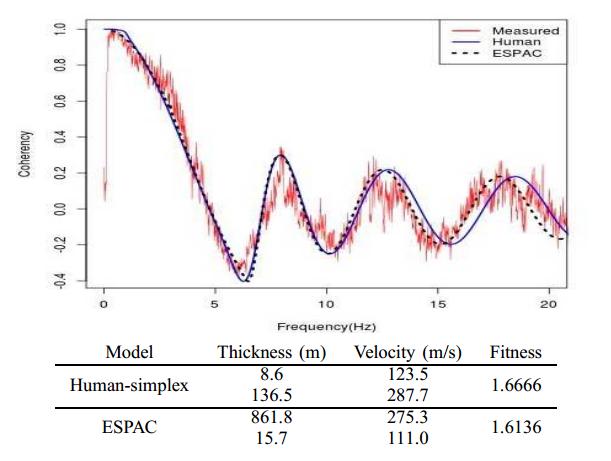
\includegraphics[width=244,height=184]{./fig1.png}
 % fig1.png: 0x0 pixel, 300dpi, 0.00x0.00 cm, bb=
 \end{center}
 \begin{center}
Fig. 1: Human and ESPAC models of a coherency curve.
\end{center}


\section*{2. The Problem}

Standard regression techniques for soil analysis are time consuming and subject to human bias. One of the most important pieces of data that needs extracting is the shear wave velocity of specific soil layers. This information is used to determine the chance a specific area has of liquefying during an earthquake event\cite{andrus1}. The development of an artificial intelligence (AI) system for increasing the performance for estimating this shear wave velocity has already
begun. \\
\\
Currently a joint Victoria University and GNS effort has produced a proof of concept
model to tackle this problem. The system uses parallel linear genetic programming and is in need of
several major performance enhancements before it can become industry viable. Currently the performance speed is very slow and the algorithms accuracy and reliability fails to pass a set of standards provided by GNS. To get this solution to an industry ready stage a substantial amount of both financial and time investment would be required. Up until
this point no alternative solutions have been investigated and it is possible that an alternative solution will
perform the task more effectively. This needs to be explored so that future resources can be allocated appropriately.
\section*{3. Proposed Solution}

This project plans to develop and evaluate five alternative AI techniques against the
existing parallel linear genetic programming solution. These techniques are:

\begin{itemize}
\item {\bf GP} Genetic programming 
\item {\bf LGP} Linear genetic programming 
\begin{itemize}
\item Both GP and LGP fit well to the nature of the problem's soil layers and the fitting of Bessel functions using symbolic regression\cite{poli1}.
\end{itemize}
\item {\bf CGA} Compact genetic algorithm 
\begin{itemize}
\item CGA is fast approach that will attempt to optimize the speed results of the GP and LGP algorithms\cite{harik1}.
\end{itemize}
\item {\bf CMA-ES} Covariance matrix adaptation evolution strategy 
\begin{itemize}
\item CMA-ES has a proven ability to deal with multi-modal\cite{hansen1} and noisy functions\cite{hansen2}.
\end{itemize}
\item {\bf LCS} Learning classifier system 
\begin{itemize}
\item This technique inclusion will be subject to the time requirements of the first 4. Should there be sufficient time this technique is a compliment to both GP and LGP presenting human readable results\cite{lanzi1}.
\end{itemize}
\end{itemize}
\\
The project will be broken down into the following stages:

\begin{description}
\item{\bf Stage 1 -} This will primarily be research into the problem itself.This includes the physical science behind it and the algorithms mentioned above. While a portion of this will be continuous throughout the project the bulk should be completed by 22 April with a presentation given to GNS around this time.
\item{\bf Stage 2 -} Each of the above techniques will then be further investigated to determine
their fit for the proposed problem. This is to remove any redundancy and avoid complication during stage 3. This should be completed by 10 May with the completion of a 5 page report.
\item{\bf Stage 3 -} The third task will be determining the evaluation methods
used to benchmark the success of each technique. A fitness function for the given problem will be determined
using the pre-existing work and communication with a geotech at GNS. This should be completed by 19 July by GNS acceptance of the documented methods.
\item{\bf Stage 4 -} The techniques that meet the problems criteria will then be
developed in Java and tested against existing benchmarks/standards a number of times to ensure statistical confidence. These results will be collated into an appendix by 8 September, this will be attached to the final report.
\item{\bf Stage 5 -} The evaluation techniques that were developed during stage 3 will then be tested against the remaining algorithms and the existing parallel linear genetic programming solution. Again these tests will be run multiple times to ensure statistical confidence and be written into an appendix by 27 September.
\item{\bf Stage 6 -} The final stage will be to ensure all the resources used and developed during the project are in a presentable format. This includes a written report, oral presentation and a tidy code repository for any future work.
\begin{description}
\item{ Written Report - 18 October(estimation only)}
\item{ Oral Presentation - 16 November(estimation only)}
\item{ Tidy Code Repository - 16 November(estimation only)}
\end{description}
\end{description}



\section*{4. Evaluating your Solution}

The success of the project will be determined by the successful implementation
of the above techniques and their evaluation against the existing system. The exact
evaluation methods will be determined during stage 3. Below is an example of the criteria that may be measured:

\begin{itemize}
 \item Fitness data measured using the results crossing points and the quadratic mean will be evaluated and compared with the parallel linear genetic programming technique.
 \item Time taken to compute compared with the parallel linear genetic programming technique.
\end{itemize}


\\
Should one of the methods
outperform the existing system a further set of evaluation methods will be
employed to determine the following (These are likely to be out of scope):
\begin{itemize}
 \item Time taken to compute against a human operator.
 \item Fitness function against a human operator.
 \item Confidence in data as determined by GNS.
\end{itemize}

\\
\\
The project should upon its completion lend strength to the argument that parallel linear genetic programming is the correct solution to the problem, or find that an alternative method would be more viable.

\section*{5. Ethics and Resourcing}


\subsection*{Ethics}
Ethics approval for this project will not be required. 

\subsection*{Safety}
There are no safety concerns for this project
successfully
\subsection*{Budget}
A transportation expenditure for George Davie will be incurred to facilitate
meetings with GNS in Avalon.
\\
\\
Access to a vehicle is available. The default mileage rate for a motor vehicle is 77 cents per kilometer(Inland Revenue)\cite{ird1}. 
\\Kelburn to Avalon return trip is 42 kilometers.
\\Estimation of 8 meetings during the course of the project.
\\{\bf 8 X 42 X 77 = \$258.72}
\\Which is preferable to -
\\Wellington Combined taxi estimation- 
\\Victoria University Kelburn - Avalon - \$80 one way 
\\5 return trips = \$800
\\
\\
{\bf Total \$258.72}
\subsection*{Space and Access}

This project will need access to a personal computer, software packages and a
computing grid that can all be found within the Engineering and Computer Science
school at Victoria University.
\\
\\
Access to Will Browne as a project supervisor will be needed at a minimum of once
per week with the provision that he can dedicate some additional time to the
review of work.
\\
\\
GNS involvement will be required as the industry partners for this project. A
set of contact people including a geotech and a seismologist should be available
via email and available for monthly progress meetings. 

\subsection*{Intellectual Property}
A standard Victoria University Intellectual Property agreement will be signed by both student George Davie and supervisor Will Browne. 
%%%%%%%%%%%%%%%%%%%%%%%%%%%%%%%%%%%%%%%%%%%%%%%%%%%%%%%
\backmatter
%%%%%%%%%%%%%%%%%%%%%%%%%%%%%%%%%%%%%%%%%%%%%%%%%%%%%%%

\bibliographystyle{ieeetr}
%\bibliographystyle{acm}
\bibliography{biblio}

\end{document}